\section{Use Case}
Based on this data model, we can represent the use cases that will allow us to test the queries:
    \begin{enumerate}
    \item on a single table with projections ($\prod$) and restriction criteria ($\sigma$)
    \item on multiple tables using joins ($\bowtie$) and restriction criteria ($\sigma$)
    \item using set queries ($\cup, \cap, \ $ )
    \item with a relational division ($\div$)
    \item applying aggregate functions (count(), sum(), max(), min(), avg() ...)
    \item performing groupings (GROUP BY)
    \item then groupings with restriction criteria (GROUP BY ... HAVING)
    \end{enumerate}

\subsection{Information Retrieval}
Using this company management model, we could implement the following use cases:
\begin{enumerate}
    \item $\prod$, $\sigma$: the name of all teams with a budget greater than €6000.00
    \item $\prod$, $\bowtie$, $\sigma$: the height of all cyclists in the "Vendée U" team
    \item $\cup$, $\cap$, \ : the name of the sponsors of the "Vendée U" team that do not have retail as their business domain
    \item $\div$: the stage where all the cyclists of the "Vendée U" team would be ranked
    \item count(), sum(), max(), min(), avg() ... : the average total distance of the races
    \item GROUP BY: the number of rankings per cyclist of the "Vendée U" team
    \item GROUP BY, HAVING: the number of rankings per cyclist of the "Vendée U" team when this number is greater than 3
\end{enumerate}
\begin{enumerate}
    \item The name of all teams with a budget greater than €6000.00
        \begin{itemize}
            \item Relational Calculus:
                \begin{itemize}
                    \item E = \{(e.name) | e $\in$ team $\wedge$ e.budget > 6000.00\}
                \end{itemize}
            \item Relational Algebra:
        	\begin{itemize}
	            \item E = $\prod_{(name)} ( \sigma_{[ budget > 6000.00]} (team) )$
	        \end{itemize}
            \item Query Tree:
            \begin{figure}[H]
            \begin{center}
            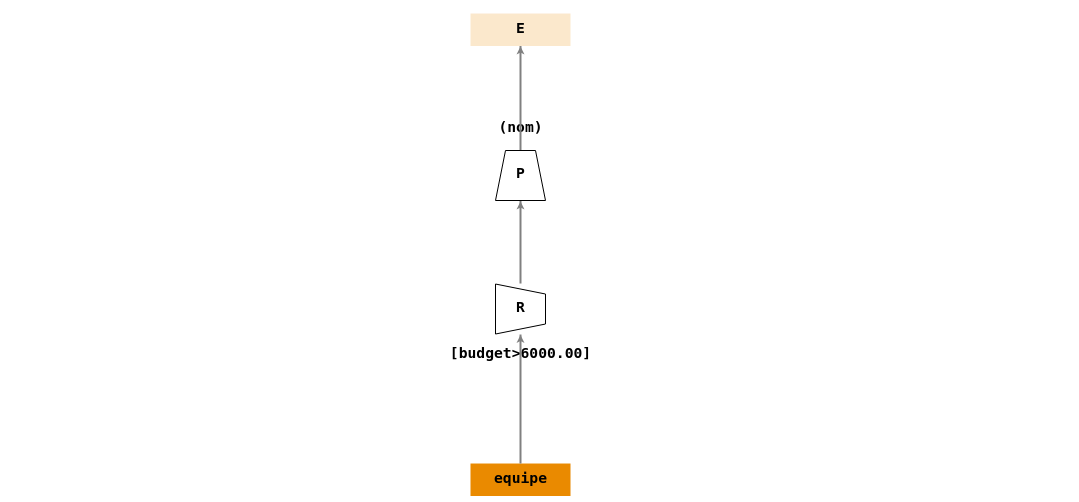
\includegraphics[height=7cm]{arbReq1.jpg}\\
            \end{center}
            \end{figure}
            \item SQL Query:
            \lstinputlisting[language=SQL]{sql/req1.sql}
        \end{itemize}

    \item The height of all cyclists in the "Vendée U" team
        \begin{itemize}
            \item Relational Calculus:
                \begin{itemize}
                    \item E1: The "Vendée U" team
                    \item E1 = \{e.rowid | team(e) $\wedge$ e.name = 'Vendée U' \}
                    \item E = \{c.height | cyclist(c) $\wedge$ E1(e1) $\wedge$ c.team\_id = e1.rowid\}
                \end{itemize}
            \item Relational Algebra:
                \begin{itemize}
                    \item E1: The "Vendée U" team
                    \item E1 = $\prod_{(rowid)} ( \sigma_{[name=Vendée U]} (team) )$
                    \item E = $\prod_{(c.height)} ( \bowtie_{[c.team\_id = E1.rowid]} (cyclist\;c, E1) )$
                \end{itemize}
            \item Query Tree:
            \begin{figure}[H]
            \begin{center}
            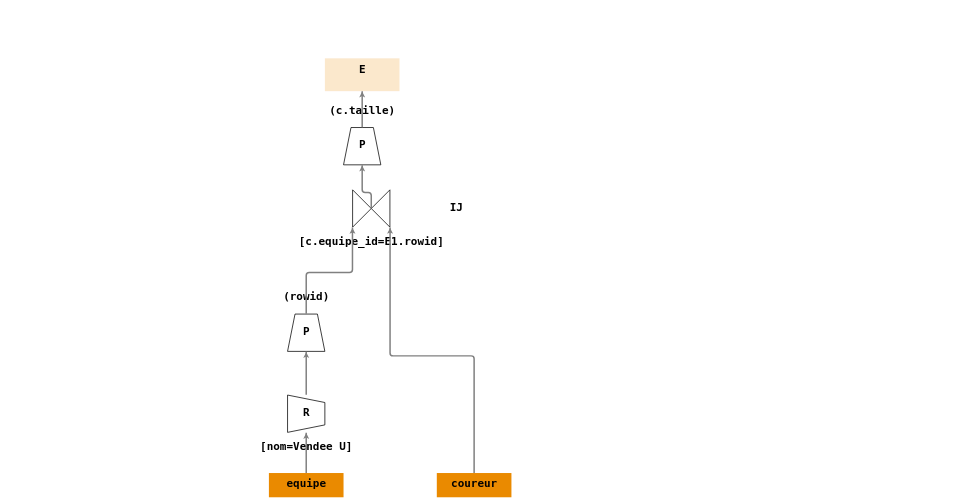
\includegraphics[height=7cm]{arbReq2.jpg}\\
            \end{center}
            \end{figure}
            \item SQL Query:
            \lstinputlisting[language=SQL]{sql/req2.sql}
        \end{itemize}
\end{enumerate}
